\section{Equipment and Supplies}

\subsection{Instrumentation}
\begin{enumerate}
    \item \href{https://www.bruker.com/products/infrared-near-infrared-and-raman-spectroscopy/ft-ir-routine-spectrometers/tensor/overview.html}{TENSOR II FTIR Spectrometer}
    \item Computer with Windows operating system and \href{https://www.bruker.com/products/infrared-near-infrared-and-raman-spectroscopy/opus-spectroscopy-software/base-package/features.html}{OPUS Spectroscopy Software} installed.
\end{enumerate}

The TENSOR II FTIR Spectrometer (Figure \ref{FTIRphoto}) has a spectral range of mid-IR 8,000-340 $cm^{-1}$, a spectral resolution of better than 0.4 $cm^{-1}$, wave number accuracy of better than 0.01 $cm^{-1}$, photometric accuracy of better than 0.1\% T, and scan velocities of 1.6 to 60 kHz. The MIR source is a U-shaped silicon carbide piece that emits mid-infrared light. The beamsplitter material is KBr, the detector used is a liquid nitrogen-cooled mercury cadmium telluride (MCT) detector. The laser is a semiconductor VCSEL diode outputting a wavelength of 850 nm at a power of 2 mW.

Technical details are available online at \href{https://www.bruker.com/products/infrared-near-infrared-and-raman-spectroscopy/ft-ir-routine-spectrometers/tensor/technical-details.html}{Bruker.com/Products} and the specifications are available in Appendix A of the TENSOR II User Manual\cite{Bruker1}.

\begin{figure}[htb]
\begin{center}
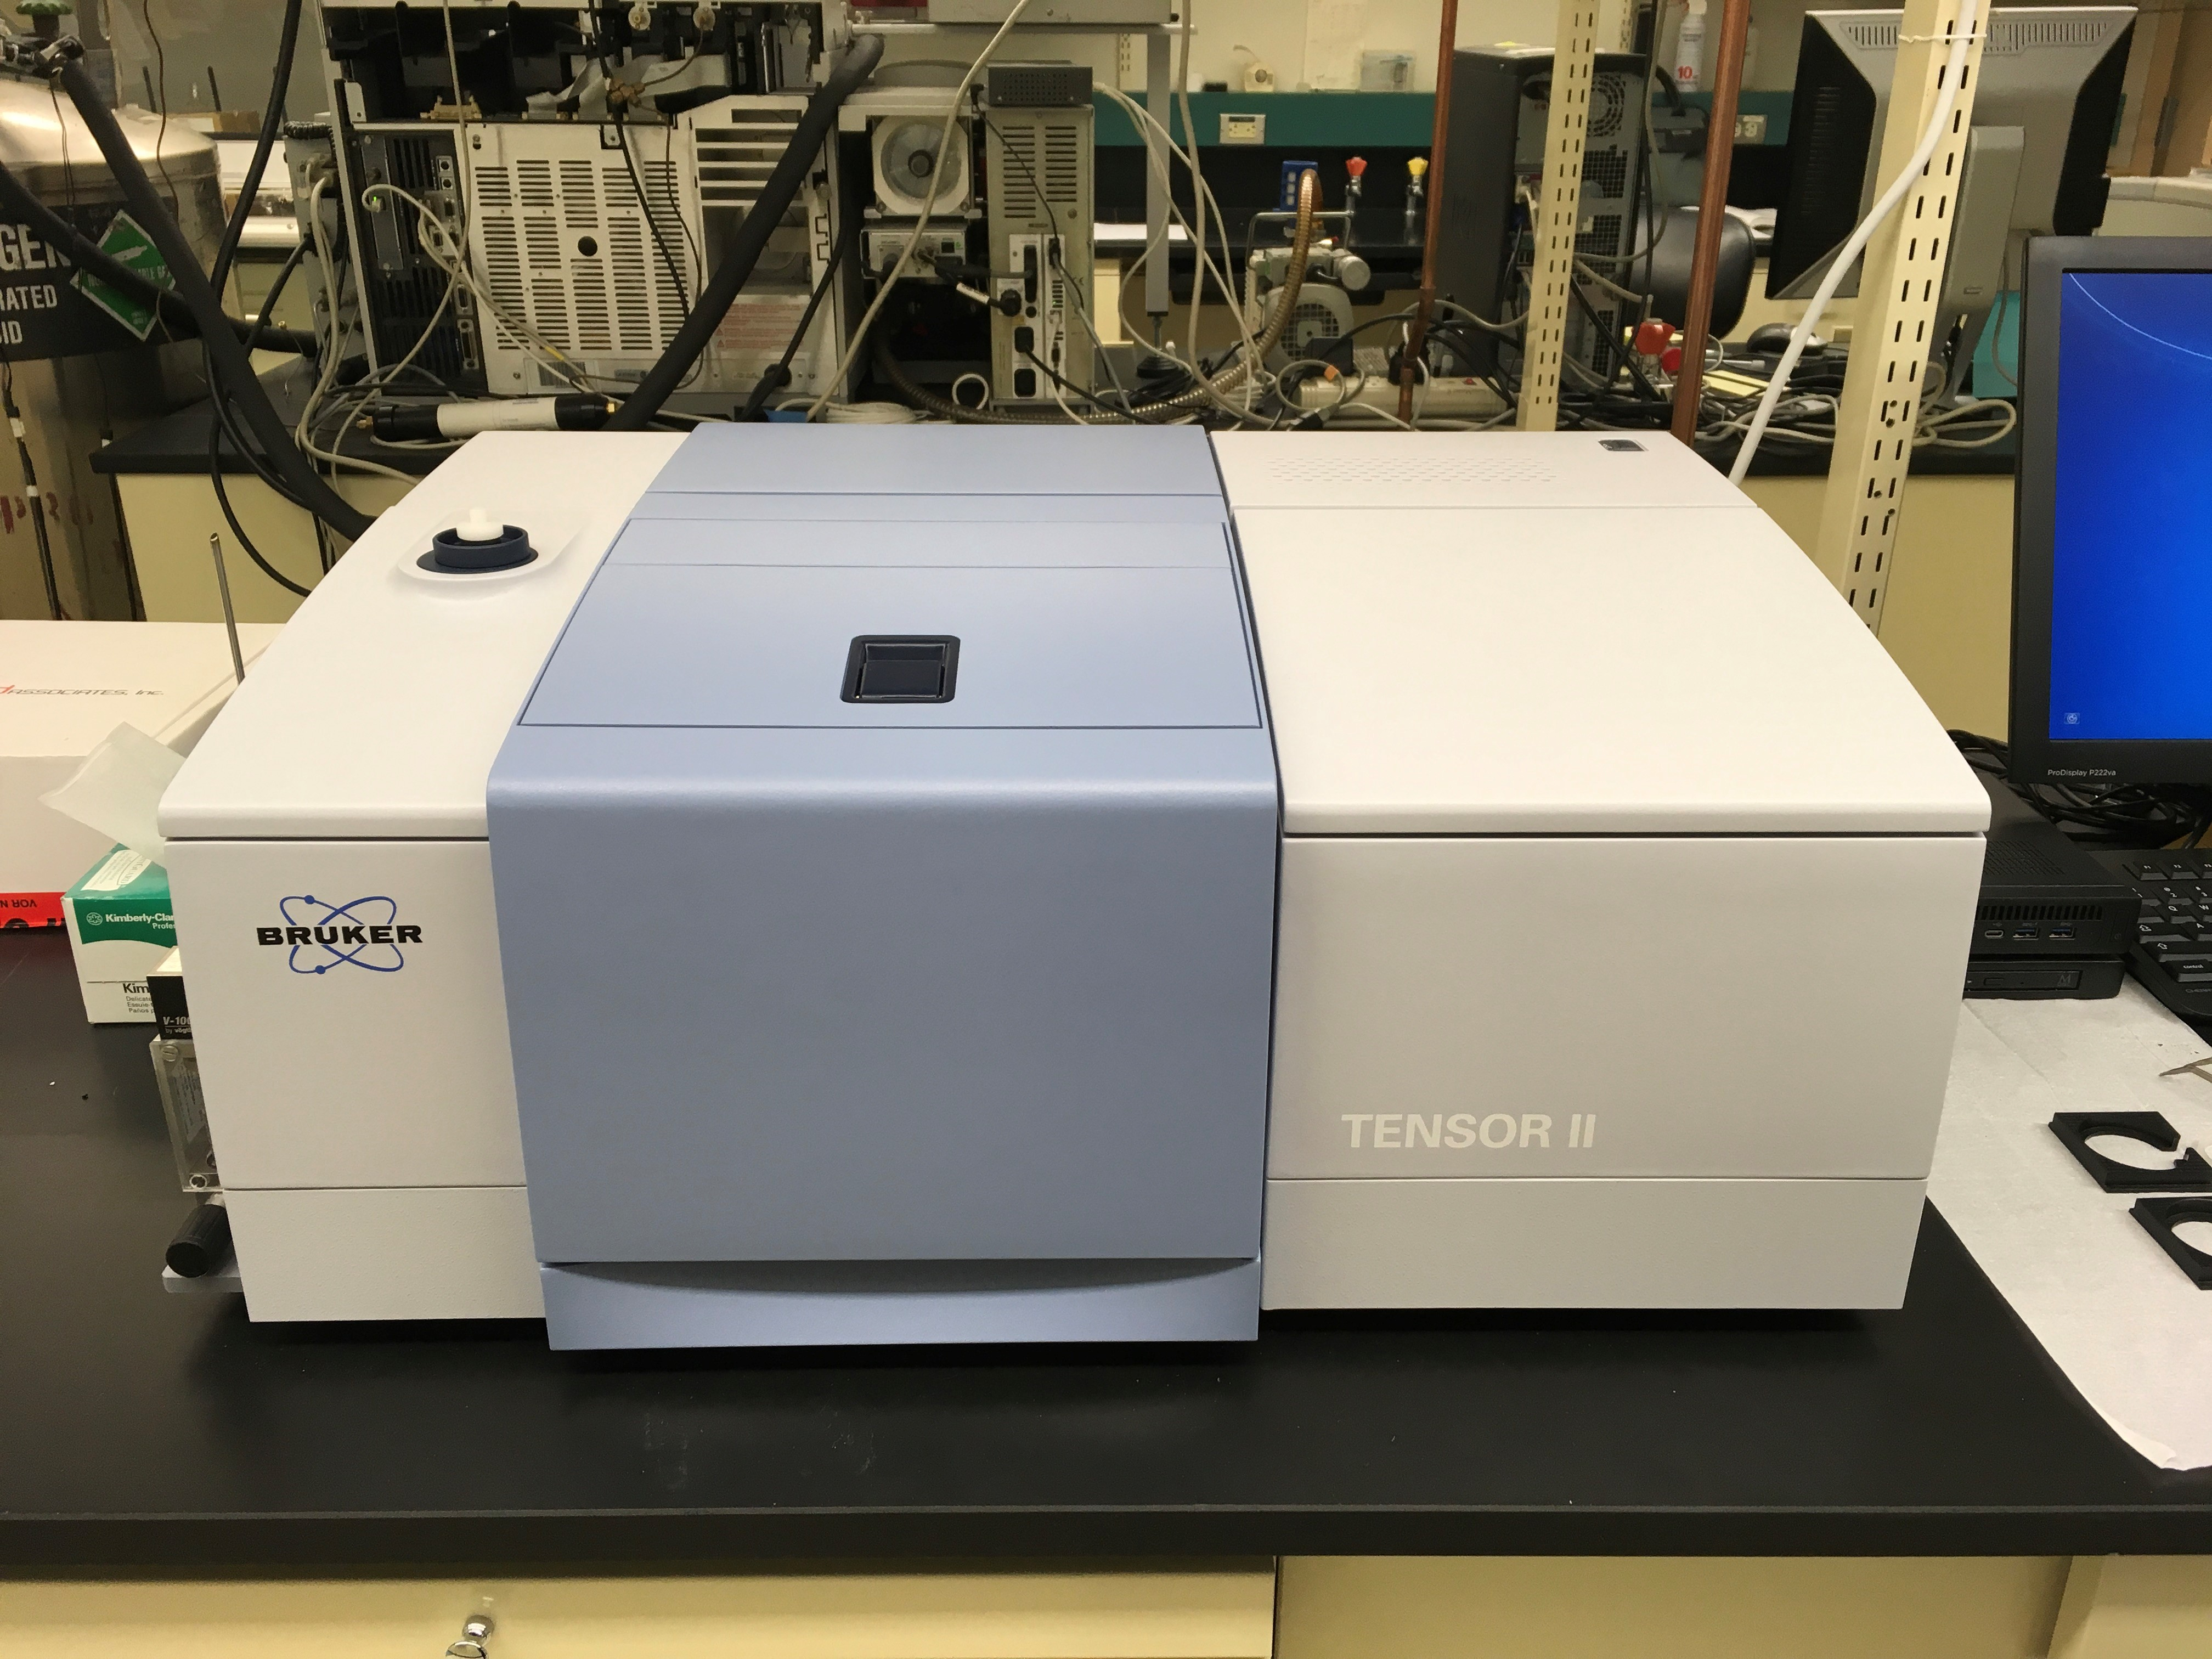
\includegraphics[width=6.5in]{TENSOR.jpg}
\caption{FT-IR instrument.}
\label{FTIRphoto}
\end{center}
\end{figure}

\subsection{Installation}
The TENSOR II is a benchtop FT-IR spectrometer capable of measuring light absorption over the IR wavelength range. Initial instrument installation was performed by the manufacturer; refer to the hardware manual (TENSOR II User Manual, saved as a PDF to the desktop of the computer installed with the TENSOR II FT-IR in lab E580A) for detailed instructions if the instrument needs to be connected to a new computer.

\subsection{Maintenance}
Components with a limited service lifetime are the IR source lamps and the desiccant cartridge.

The interferogram peak test and the energy test described in Section \ref{subsec:individualPQ} on page \pageref{subsec:individualPQ} can be used to determine whether the IR source lamp needs to be replaced.

The desiccant cartridge in the TENSOR II interferometer should be replaced every 6 months\cite{Bruker1}. Refer to the TENSOR II User Manual Section 6.3 Replacing the cartridge and regenerating the desiccant.

Refer to the TENSOR II User Manual for troubleshooting procedures and replacement part numbers.

The spectrometer sample compartment and sample holder should be kept clean. %In the case of a spill:
%\begin{enumerate}
%    \item Remove the sample holder by removing the ... (Figure \ref{holderremoval})\todo{show proprietary sample holder?}.
%\begin{figure}[h]
%\begin{center}
%\includegraphics[width=]{}
%\missingfigure{Sample holder removal}
%\caption{Close-up of compartment showing sample holder removal.}
%\label{holderremoval}
%\end{center}
%\end{figure}
%    \item Clean surfaces with Kimwipes and ethanol or isopropanol.
%    \item Allow to dry before reinstalling the holder.
%    \item Reinstall the sample holder by placing the holder on...
%\end{enumerate}



\subsection{Ancillary equipment: purge gas supply}
An \href{http://www.ekom.sk/en/products/industrial-compressors/mobile-compressors/industrial-compressor-dk50-plus-mobile/}{ekom\textsuperscript{\textregistered} DK50 PLUS/M MOBILE combination air compressor and dehumidifier} acts as the purge gas supply for the TENSOR II FT-IR Spectrometer. %A technical leaflet PDF is available at \url{http://www.ekom.sk/fileadmin/ekom/prospekty/jednolistovky/rok_2015_aplikacie/2016/aplik_EN_DE_FR_2016_16_dk50_plus_mobile.pdf}.

A \href{https://www.voegtlin.com/en/variable-area-flowmeters-and-control-valves/va-flowmeters-v-100/}{V\"{o}gtlin V-100 55 variable area flow meter} is used to control the purge gas flow rate. The datasheet PDF is available at \url{https://www.voegtlin.com/data/139-2018_en_infoV100.pdf}.

The purge gas supply is plumbed to the FT-IR spectrometer as shown in Figure \ref{FTIRgas}.
\begin{figure}[htb]
\begin{center}
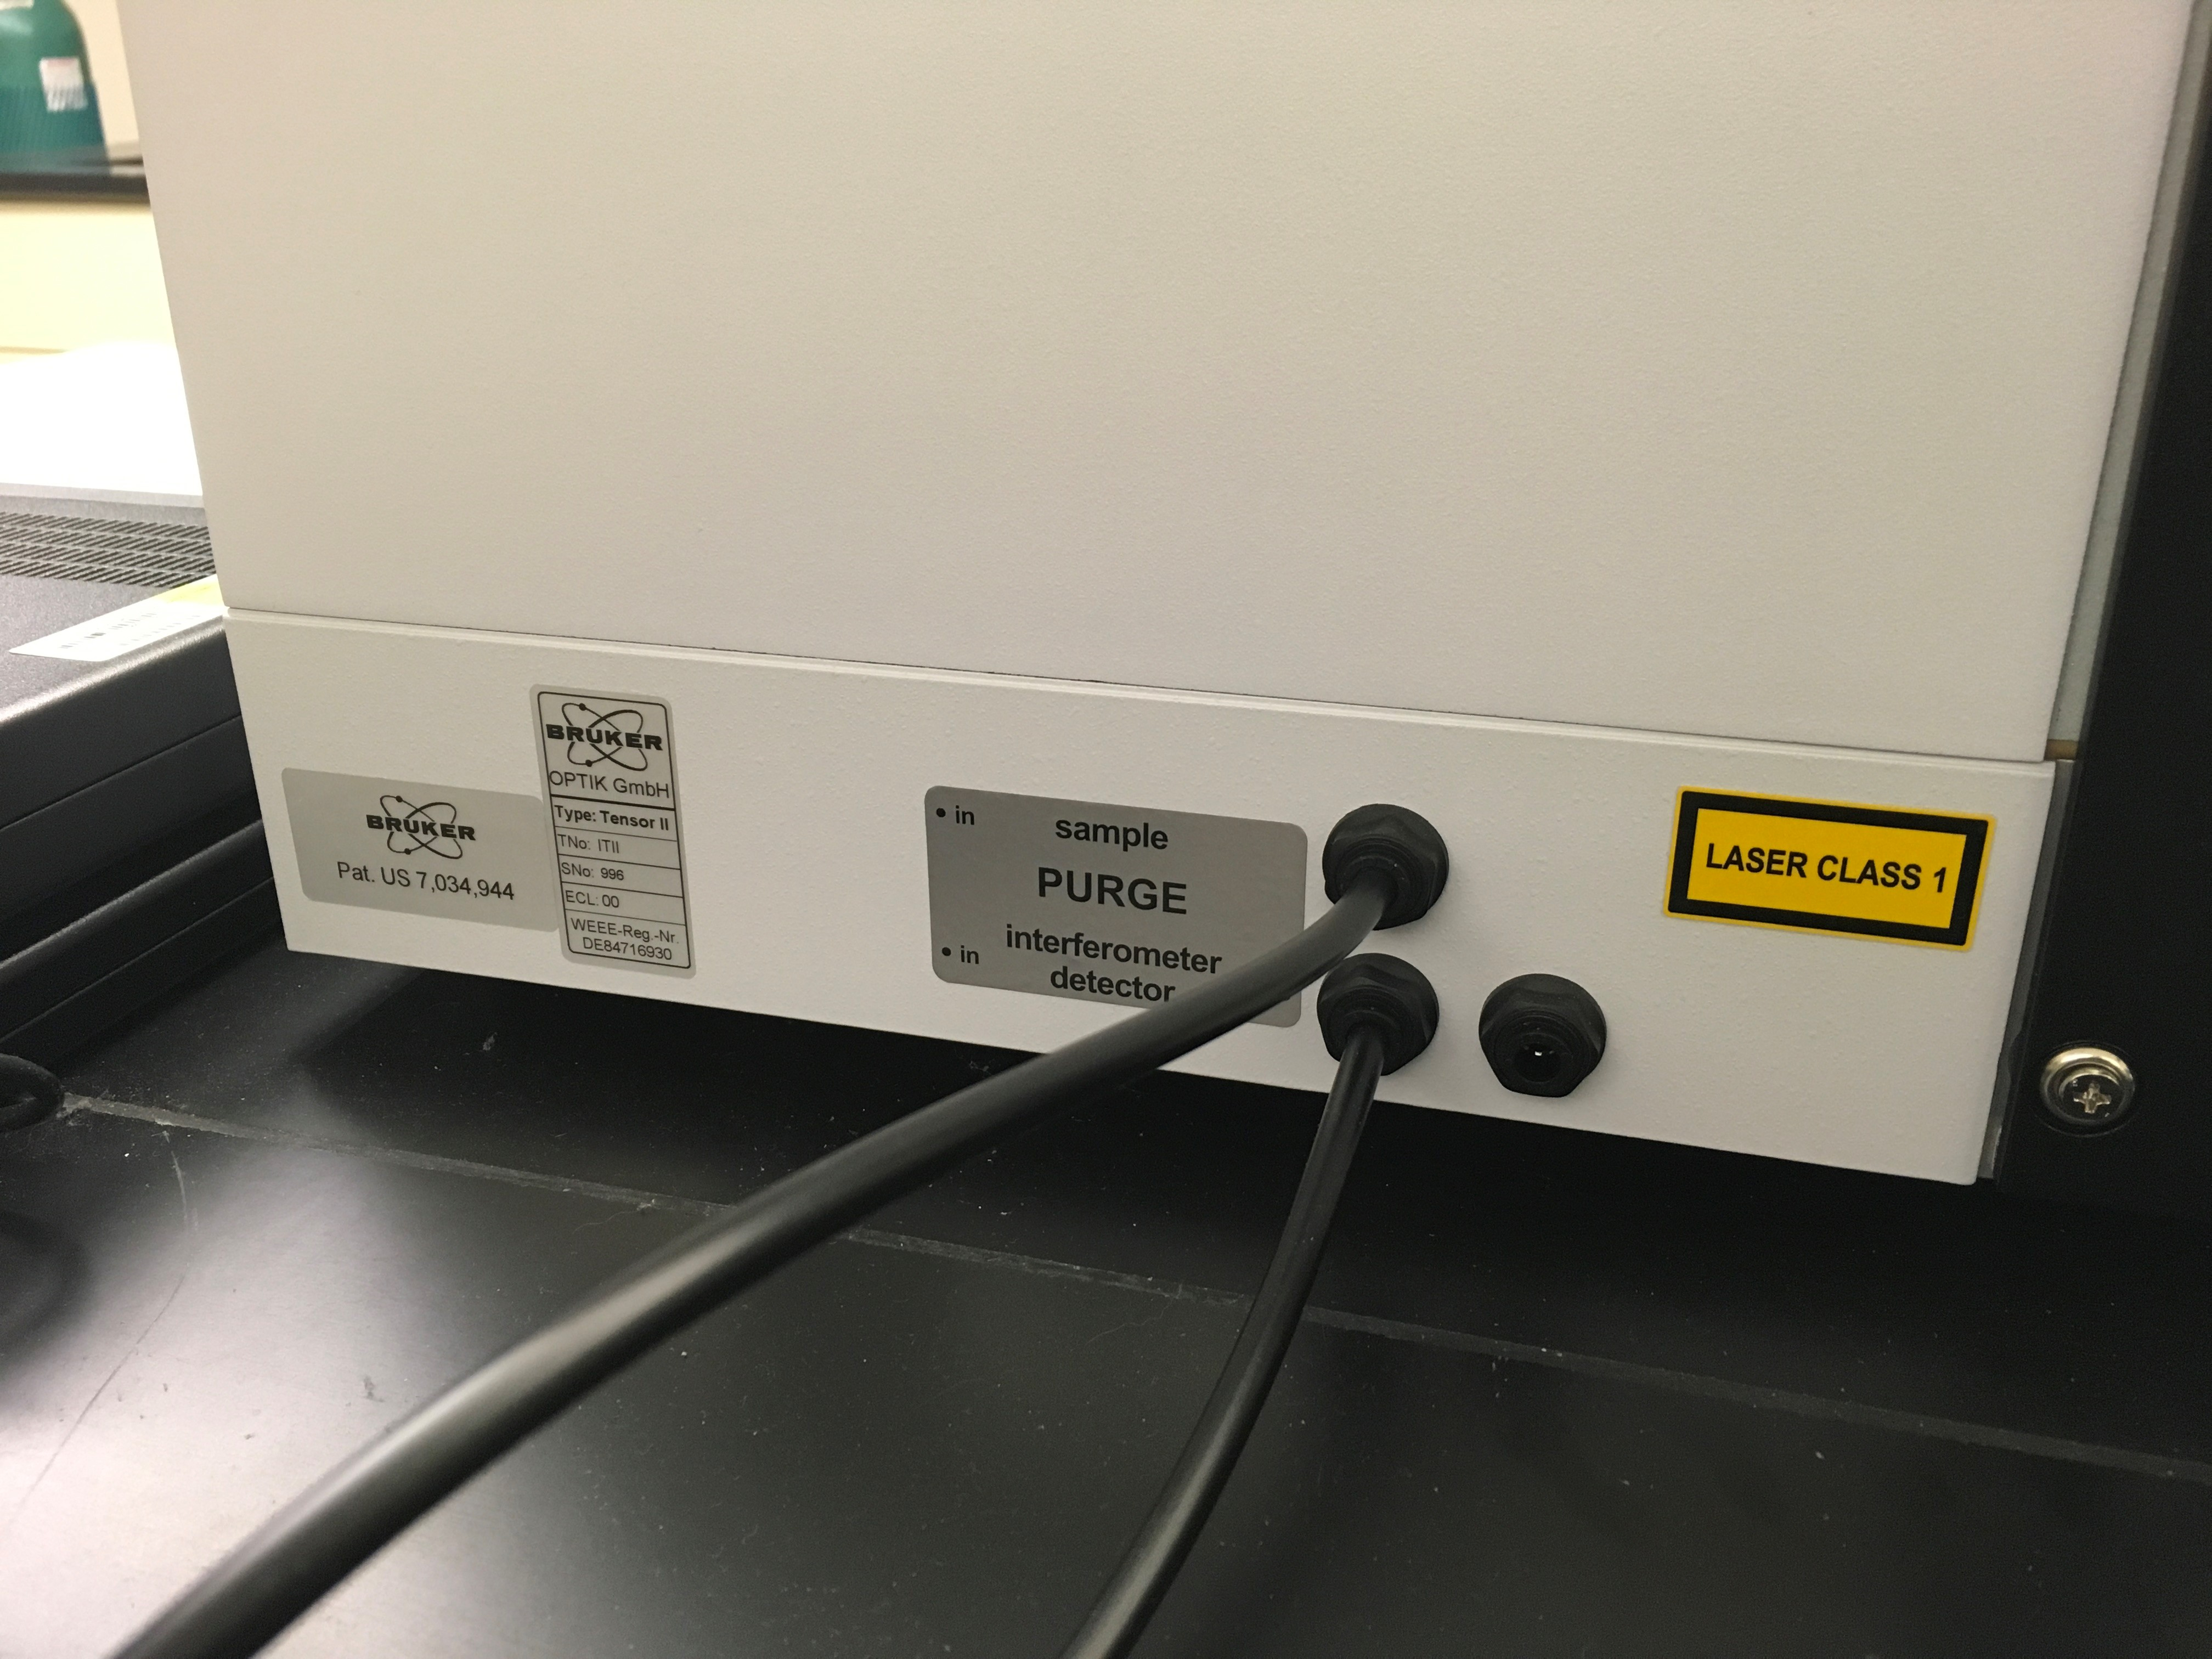
\includegraphics[width=6.5in]{purgeplumbing.jpg}
\caption{Back of the TENSOR II FT-IR, showing where the purge gas supply is plumbed into the spectrometer housing.}
\label{FTIRgas}
\end{center}
\end{figure}

Use the following specifications as stated by the TENSOR II User Manual to purge the optical bench and sample compartment in the TENSOR II FT-IR\cite{Bruker1}:
\begin{itemize}
    \item Dry air (with a dew point $<-40^\circ C$, which corresponds to a degree of dryness of 128ppm humidity)
    \item Oil-free and dust-free
    \item Maximum pressure: 2 bar (29 psi)
    \item Recommended sustained purge gas flow rate: 200 liters/hour
    \item The purge gas flow rate should not exceed 500 liters/hour. Too high a purge gas flow rate will both damage the optics and introduce acoustic noise into measurements.
\end{itemize}

\subsection{Sample requirements}
Sample collection will be covered by the separate quality assurance plan. This QAPP covers the measurement of filter samples. 

Air filters used with this FT-IR measurement procedure must be Teflon or polytetrafluoroethylene (PTFE) membrane disc filters of circumference 25, 37, or 47 mm. The membrane pore sizes must be 1, 2, or 3 microns. Acceptable brands include Pall Corporation and MTL, LLC.